\chapter{Heap}
\section{Definition}
	A heap is a \textbf{binary} tree with two properties:
	\begin{itemize}
		\item Shape: Its shape must be complete. All of the nodes from all the levels must be filled, except the last one.
		\item Order: It must have all of its nodes in a specific order.
		\begin{itemize}
			\item \textbf{Min-Heap}: A heap's root node must have of its children be either smaller than or equal to it's children.
			\item \textbf{Max-Heap}: A heap's root node must have of its children be either greater than or equal to it's children.
		\end{itemize}
	\end{itemize}
\section{Basics}
	\begin{itemize}
		\item We can always have duplicates in a heap
		\item Heaps don't follow the binary search tree rule that the left node needs to be smaller than the right.
		\item No matter if we grow or shrink the heap, we must always maintain it's two properties
		\item It's used in a system scheduler where a priority queue will say which task should be executed next (task, item with highest priority will be dequeued from the heap)
	\end{itemize}
	\section{Storing a Heap}
	\begin{figure}[H]
		\centering
		\scalebox{0.40}
			{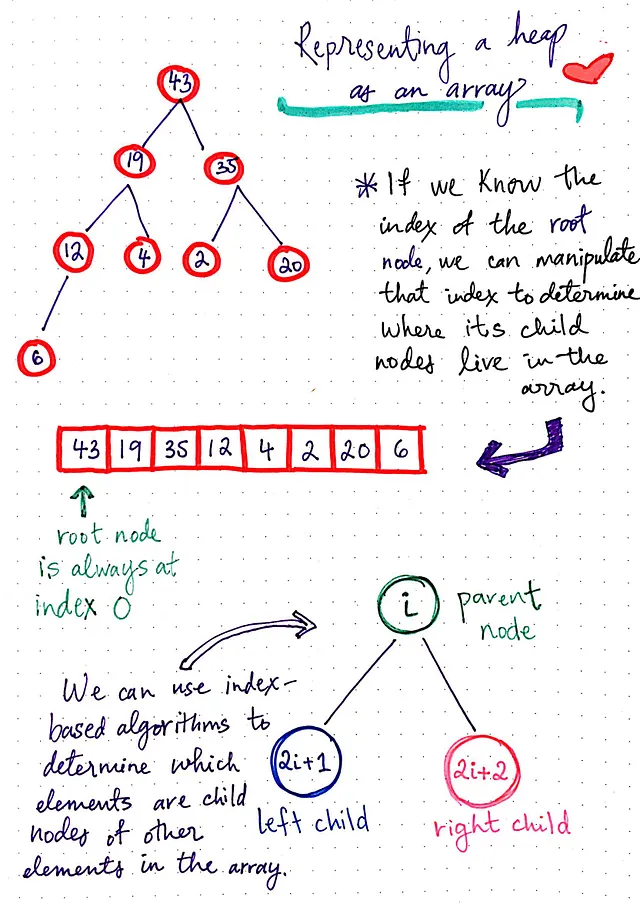
\includegraphics{images/heap_1}}
		\caption{Heap as an array structure}
	\end{figure}	
	
	\section{Getting the heap out of the Array}
	\begin{figure}[H]
		\centering
		\scalebox{0.40}
			{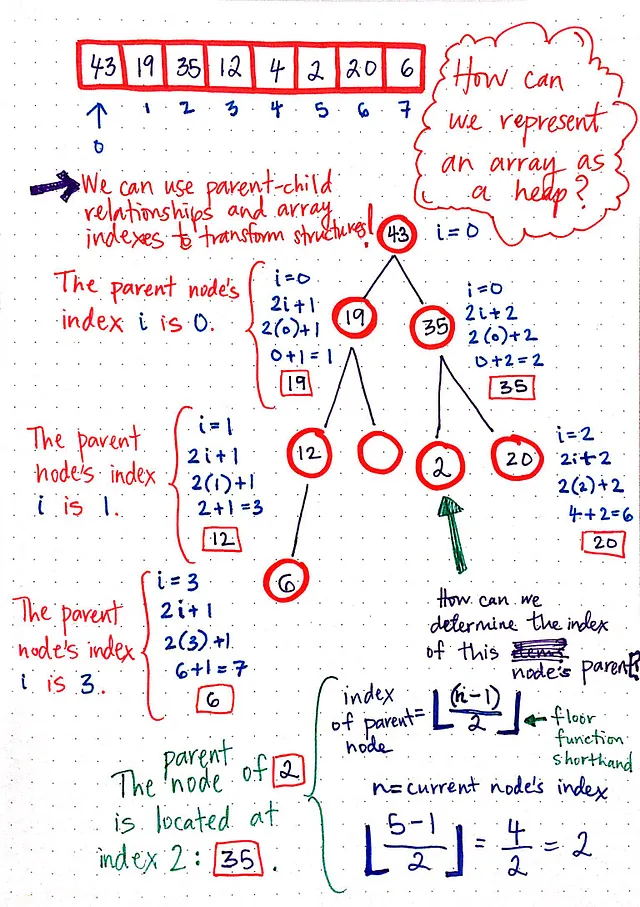
\includegraphics{images/heap_2}}
		\caption{Heap as an array structure}
	\end{figure}	
	
	\section{Heap Sort Algorithm}
		\begin{itemize}
			\item Improved Selection Sort with O(nlogn) time complexity
			\item buildMaxHeap()
			\item heapify()
		\end{itemize}

	\section{Corner Cases}
		\begin{itemize}
			\item Empty stack. Popping from an empty stack
			\item Stack with one item
			\item Stack with two items
		\end{itemize}
		
	
	\section{Time complexity}
	
	\begin{center}
		\begin{tabular}{||c c||}
		\hline
		Operation & Complexity\\
		\hline\hline
		Top/Peek & O(1)\\
		\hline
		Push & O(1)\\
		\hline
		Pop & O(1)\\
		\hline
		isEmpty & O(1)\\
		\hline
		Search & O(n)\\
		\hline
			
		\end{tabular}
	\end{center}
	
	
	